\begin{figure*}[ht]
    % \vspace{-5pt}
    \begin{minipage}[b]{\textwidth}
        % \begin{center}

        \subfigure[MHC aligned pangenome]{
            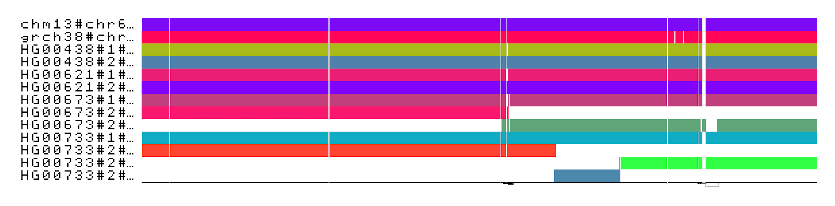
\includegraphics[width=.6\textwidth]{fig/mhc-align.eps}
            \label{fig:1a}
        }
        \vspace{-11pt}
        % \newline
        \subfigure[MHC consensus pangenome]{
            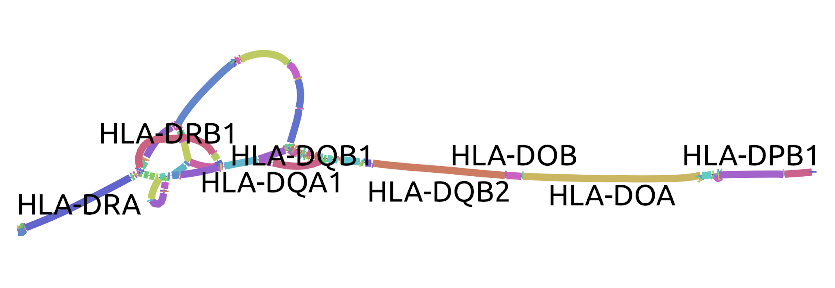
\includegraphics[width=.4\textwidth]{fig/mhc-pangenome.eps}
            \label{fig:1b}
        }
        \caption{Pangenome visualisation of the MHC \textit{locus}.
            (a) projection of full MHC \textit{locus} of haploid phased human genome
          assemblies, plus the chm13 cell line and GRCh38 reference genome as supplied by the
            HPRC and created by \cmd{odgi build+sort+viz}. The coloured
            bars represent the linearised paths --- representing contigs as a zoomed out multi-sequence
            alignment. The black lines at the bottom represent the graph topology.
            (b) consensus graph representation of the same assemblies showing variations larger than $100$ base pairs.
            Loops or `bubbles' display contigs uniquely diverging from the consensus, caused by variation in paralogs/repeats.
            The gene labels are super imposed by \cmd{odgi build+position} from a GRCh38 BED file and visualised by the
            Bandage tool~\citep{Wick:2015}.
        }
        \label{fig:1}
        % \end{center}
    \end{minipage}
\end{figure*}
